%%%%%%%%%%%%%%%%%%%%%%%%%%%%%%%%%%%%%%%%%
% Beamer Presentation
% LaTeX Template
% Version 1.0 (10/11/12)
%
% This template has been downloaded from:
% http://www.LaTeXTemplates.com
%
% License:
% CC BY-NC-SA 3.0 (http://creativecommons.org/licenses/by-nc-sa/3.0/)
%
%%%%%%%%%%%%%%%%%%%%%%%%%%%%%%%%%%%%%%%%%

%----------------------------------------------------------------------------------------
%	PACKAGES AND THEMES
%----------------------------------------------------------------------------------------

\documentclass{beamer}

\mode<presentation> {

% The Beamer class comes with a number of default slide themes
% which change the colors and layouts of slides. Below this is a list
% of all the themes, uncomment each in turn to see what they look like.

%\usetheme{default}
%\usetheme{AnnArbor}
%\usetheme{Antibes}
%\usetheme{Bergen}
%\usetheme{Berkeley}
%\usetheme{Berlin}
%\usetheme{Boadilla}
\usetheme{CambridgeUS}
%\usetheme{Copenhagen}
%\usetheme{Darmstadt}
%\usetheme{Dresden}
%\usetheme{Frankfurt}
%\usetheme{Goettingen}
%\usetheme{Hannover}
%\usetheme{Ilmenau}
%\usetheme{JuanLesPins}
%\usetheme{Luebeck}
%\usetheme{Madrid}
%\usetheme{Malmoe}
%\usetheme{Marburg}
%\usetheme{Montpellier}
%\usetheme{PaloAlto}
%\usetheme{Pittsburgh}
%\usetheme{Rochester}
%\usetheme{Singapore}
%\usetheme{Szeged}
%\usetheme{Warsaw}

% As well as themes, the Beamer class has a number of color themes
% for any slide theme. Uncomment each of these in turn to see how it
% changes the colors of your current slide theme.

%\usecolortheme{albatross}
%\usecolortheme{beaver}
%\usecolortheme{beetle}
%\usecolortheme{crane}
%\usecolortheme{dolphin}
%\usecolortheme{dove}
%\usecolortheme{fly}
%\usecolortheme{lily}
%\usecolortheme{orchid}
%\usecolortheme{rose}
%\usecolortheme{seagull}
\usecolortheme{seahorse}
%\usecolortheme{whale}
%\usecolortheme{wolverine}

%\setbeamertemplate{footline} % To remove the footer line in all slides uncomment this line
%\setbeamertemplate{footline}[page number] % To replace the footer line in all slides with a simple slide count uncomment this line

%\setbeamertemplate{navigation symbols}{} % To remove the navigation symbols from the bottom of all slides uncomment this line
}
\usepackage{amsmath}
\usepackage{graphicx} % Allows including images
\usepackage{booktabs} % Allows the use of \toprule, \midrule and \bottomrule in tables

%----------------------------------------------------------------------------------------
%	TITLE PAGE
%----------------------------------------------------------------------------------------

\title[SFC mapping]{A Novel Approach for Service Function Chain (SFC)Mapping with Multiple SFC instances in a Fog-To-Cloud Computing System} % The short title appears at the bottom of every slide, the full title is only on the title page

\author[A.Zamani]{A.Zamani\\[1mm]{\small Supervised by: Dr. Sharifian}} % Your name
\institute[AUT] % Your institution as it will appear on the bottom of every slide, may be shorthand to save space
{
Amirkabir University of Technology \\ % Your institution for the title page
}
\date[ICSPIS, December 2018]{ICSPIS Conference, December 2018} % Date, can be changed to a custom date

\begin{document}

\begin{frame}
\titlepage % Print the title page as the first slide
\end{frame}

\begin{frame}
\frametitle{Outline} % Table of contents slide, comment this block out to remove it
\tableofcontents % Throughout your presentation, if you choose to use \section{} and \subsection{} commands, these will automatically be printed on this slide as an overview of your presentation
\end{frame}

%----------------------------------------------------------------------------------------
%	PRESENTATION SLIDES
%----------------------------------------------------------------------------------------

%------------------------------------------------


\section{Introduction}
\subsection[IoT]{Internet of Things (IoT)}
\begin{frame}
\frametitle{Introduction}
\begin{itemize}
	\item IoT
	\begin{itemize}
		\item {interconnects billions or
			even trillions of diverse devices}
		\item {generate a massive
			amount of data}
		\item {should be transmitted to the cloud for
			computing}
	\end{itemize}
\end{itemize}
\begin{figure}
	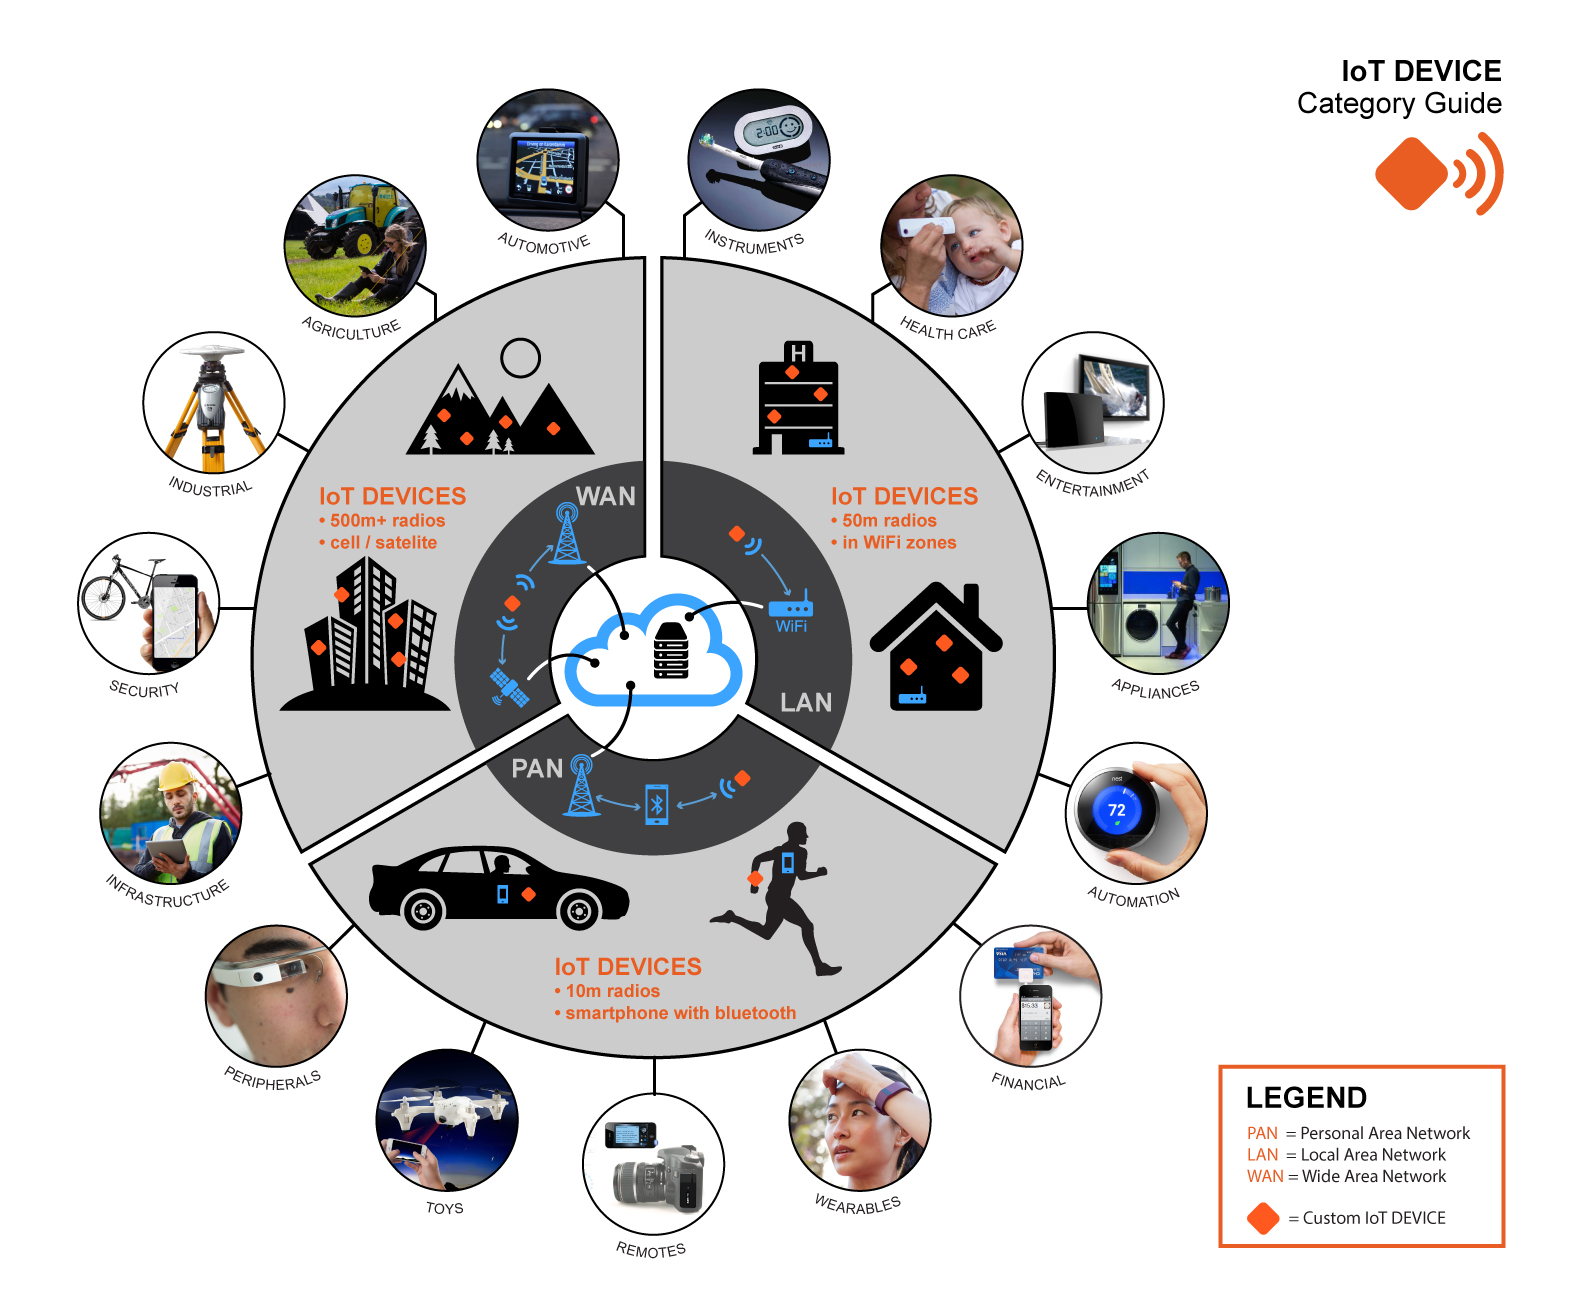
\includegraphics[scale=0.1]{IoT1}
	\caption{IoT devices}
	\label{fig:iot1}
\end{figure}
\end{frame}
\subsection{Cloud computing}
\begin{frame}
\frametitle{Introduction}
\begin{itemize}
	\item Cloud computing
	\begin{itemize}
		\item \color{blue} {cloud offers various benefits such as
			scalability and elasticity}
		\item {consolidation and centralization
			lead to many network hops}
		\item \color{red}{results in high latencies and high bandwidth consumption}
		
	\end{itemize}
\end{itemize}
\begin{figure}
	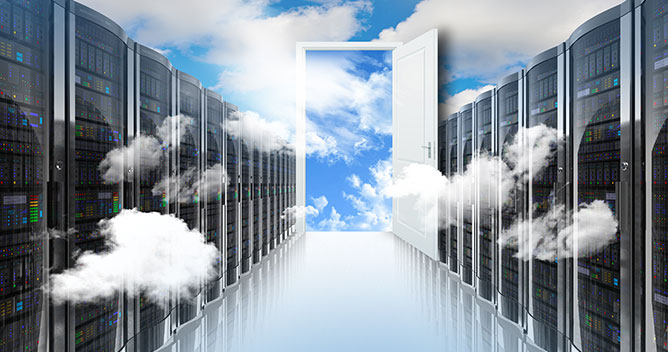
\includegraphics[scale=0.35]{cloud-computing-2}
	\caption{Cloud computing}
	\label{fig:cloud-computing-2}
\end{figure}
\end{frame}
\begin{frame}
\frametitle{Introduction}
\begin{itemize}
	\item Healthcare
\end{itemize}	
\begin{figure}
	\centering
	
\includegraphics[width=0.7\linewidth]{healthcare}
	\caption{Healthcare}
	\label{fig:healthcare}
\end{figure}
\end{frame}
\begin{frame}
\frametitle{Introduction}
\begin{itemize}
	\item Augmented reality
\end{itemize}	
\begin{figure}
	\centering
	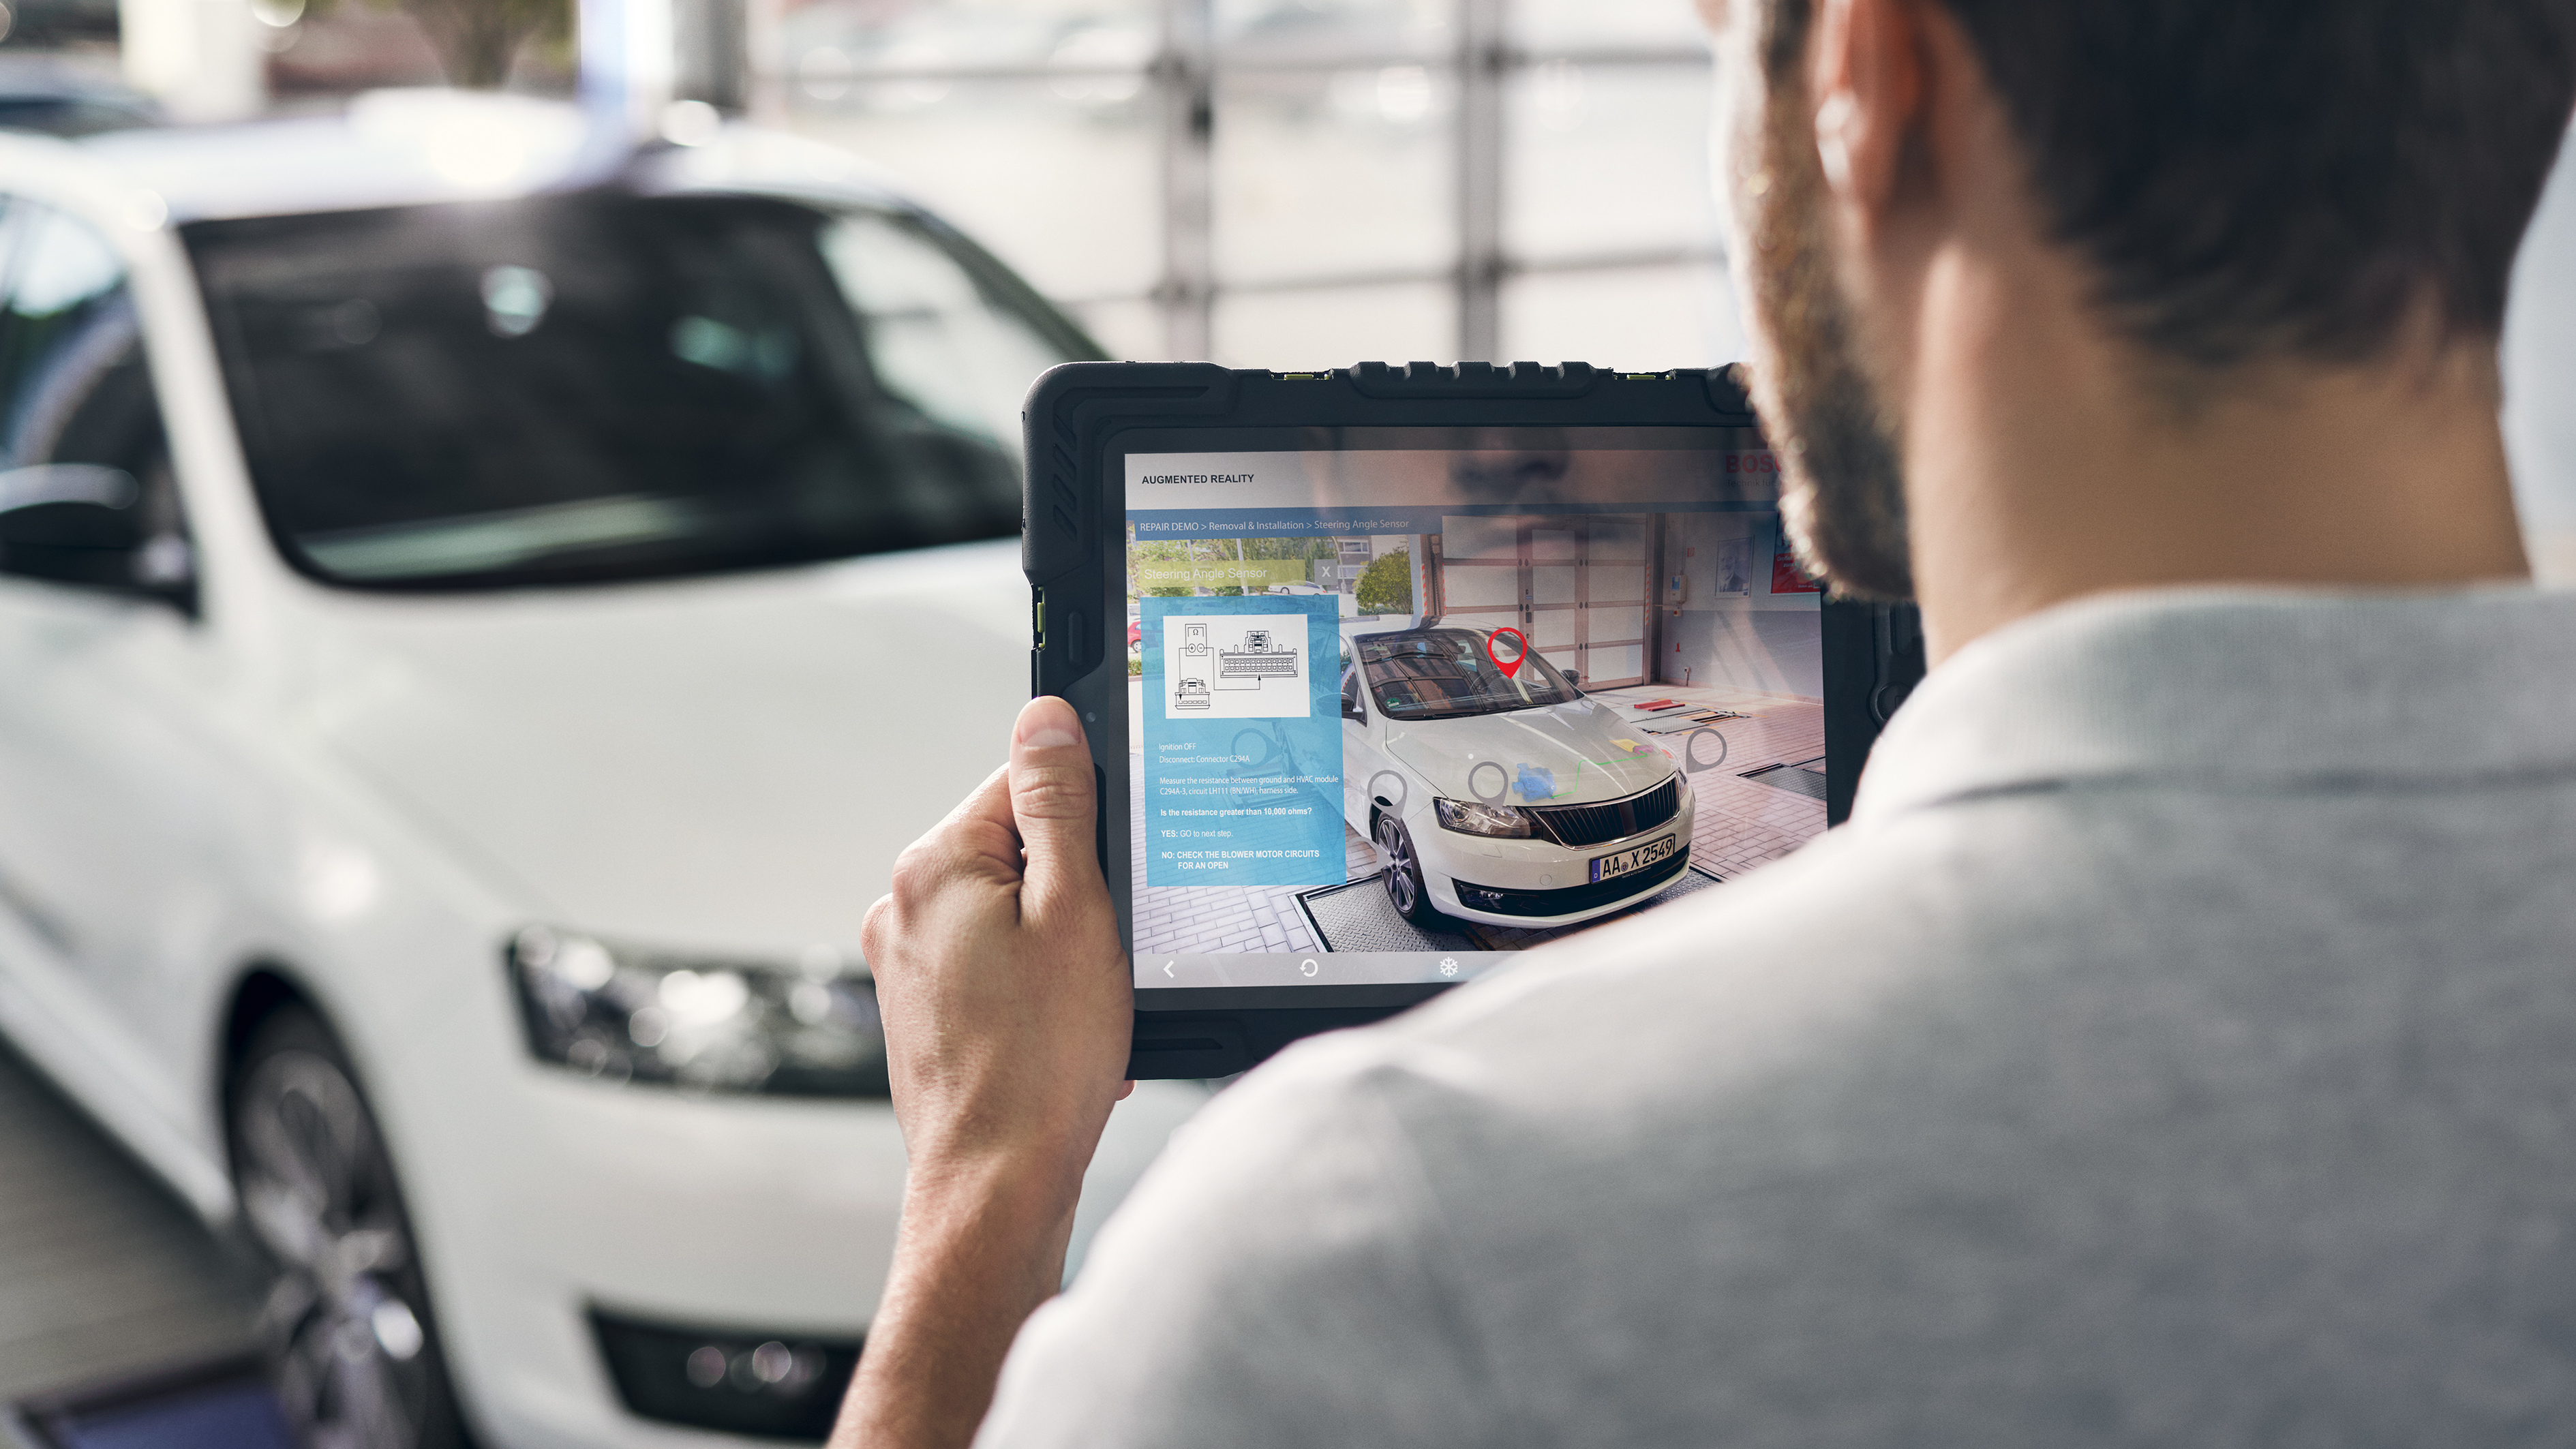
\includegraphics[width=0.7\linewidth]{agmented_R}
	\caption{Augmented reality}
	\label{fig:agmentedr}
\end{figure}
\end{frame}
\subsection{Fog computing}
\begin{frame}
\frametitle{Introduction}
	\begin{itemize}
		\item Fog computing
		\begin{itemize}
			\item<1-> {offers distributed
				edge cloud close to the Things}
		\end{itemize}
	\end{itemize}
\begin{figure}
	\centering
	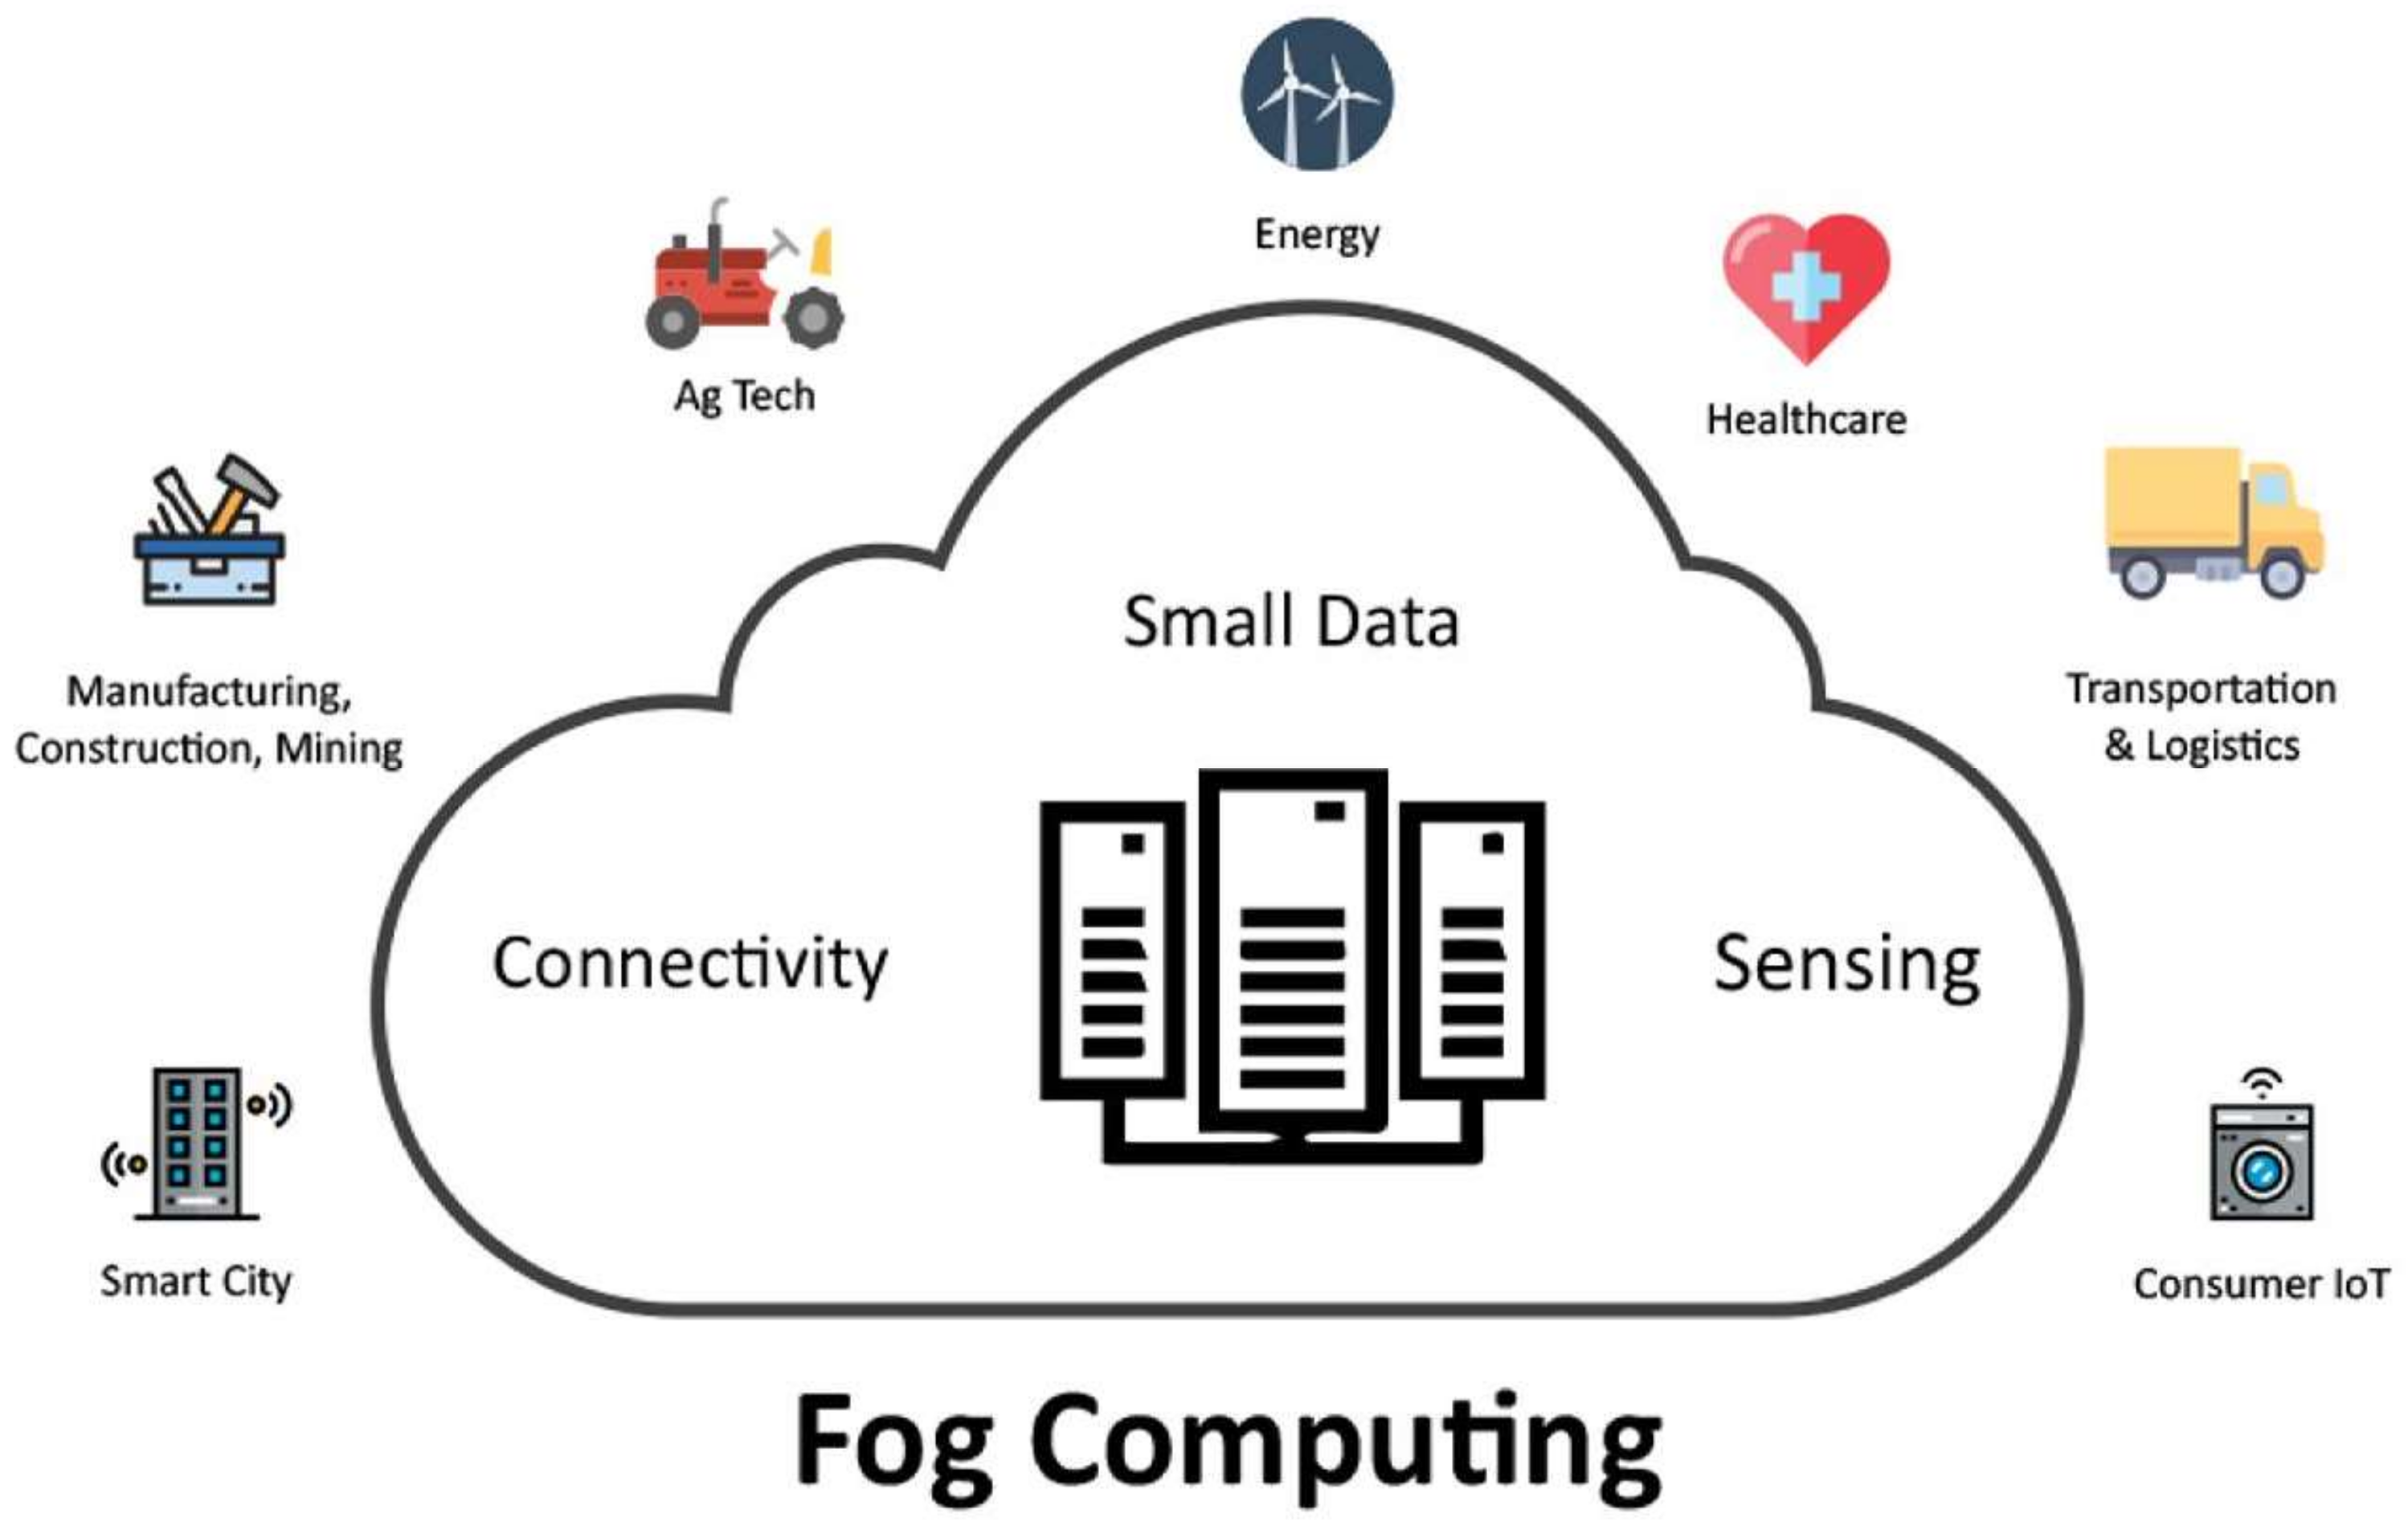
\includegraphics[width=0.7\linewidth]{fog-computing}
	\label{fig:fog-computing}
\end{figure}

\end{frame}
\subsection[Fog-to-Cloud]{Fog-to-Cloud computing system}
\begin{frame}
	\begin{itemize}
	\item Fog-to-Cloud computing system
	\begin{itemize}
		\item {fog and cloud work together}
		\item {provide computing, storage, and application servicesin the IoT domain}
		\item \color{red}{complex management of such a
			network of distributed fogs}
			
	\end{itemize}
\end{itemize}
\begin{figure}
	\centering
	\includegraphics[scale=0.13]{"Fog-to-cloud computing system"}
	\caption{Fog-to-Cloud computing system}
	\label{fig:fog-to-cloud-computing-system}
\end{figure}
\end{frame}
\subsection[SDN and NFV]{Software Defined Network and network function virtualization}
\begin{frame}
	\begin{itemize}
		\item Software Defined Network(SDN)
		\begin{itemize}
			\item {SDN separates the control and data planes}
		\end{itemize}
	\end{itemize}
\begin{figure}
	\centering
	
\includegraphics[width=0.7\linewidth]{sdn2}
	\caption{Software Defined Network}
	\label{fig:sdn2}
\end{figure}

\end{frame}	
\begin{frame}
\begin{itemize}
	\item network function virtualization(NFV)
	\begin{itemize}
		\item {NFV reshapes dedicated hardware functionality}
		\item {software modules named virtual network functions (VNFs)}
		\item \color{blue}{agile and scalable service placement}
		\item \color{blue} {reducing Capital
			Expenditure (CAPEX) and Operation Expense (OPEX)}
	\end{itemize}
\end{itemize}
\begin{figure}
	\centering
	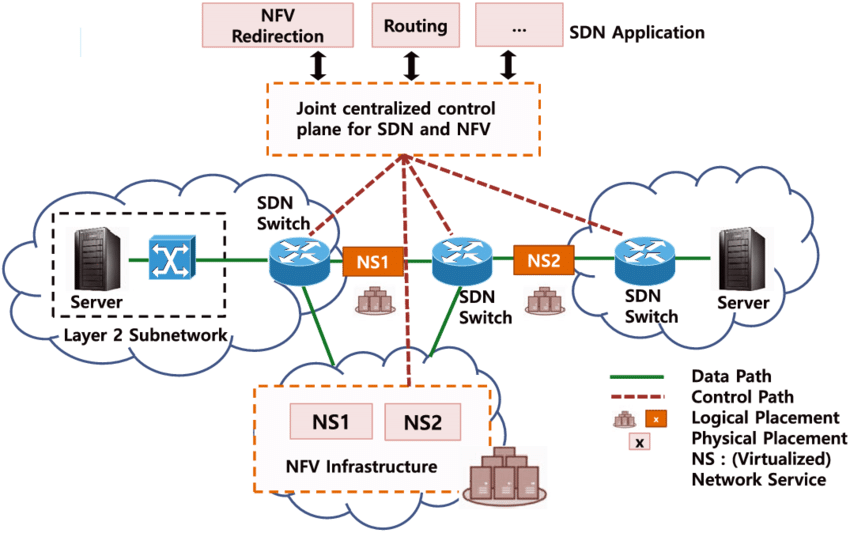
\includegraphics[width=0.62\linewidth]{Architecture-of-a-software-based-network-with-support-for-network-virtualization-NFV}
	\caption{SDN based network with support for NFV}
	\label{fig:architecture-of-a-software-based-network-with-support-for-network-virtualization-nfv}
\end{figure}
\end{frame}
\begin{frame}
	\begin{itemize}
		\item {Service Function Chaining(SFC)}	
		\begin{itemize}
			\item{specific set of VNFs}
			\item{joint VNF placement and traffic routing
				are called SFC mapping}	
		\end{itemize}
	\end{itemize}
\begin{figure}
	\centering
	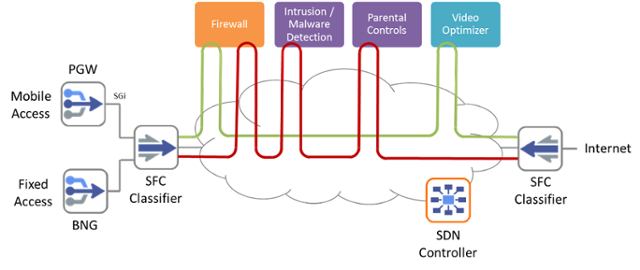
\includegraphics[width=0.9\linewidth]{sfcexample}
	\caption{Service Function Chaining}
	\label{fig:sfcexample}
\end{figure}
\end{frame}
\subsection{Related Work}
\begin{frame}
	\begin{table}
		\begin{tabular}{|c|c|c|c|c|}
			\toprule
			\textbf{Author} & \textbf{Year} & \textbf{Mapping} &\textbf{Solution}& \textbf{Objective}\\
			\midrule
			Draxler & 2017 & VNFs mapping & heuristic & total data rate \\
			 & & & and exact & and total latency\\
			 \hline
			 Huin &2018 & Placement& exact &total latency\\
             \hline
             Masri&2017& Select optimal  &exact &total latency\\
              & & fog or cloud& & \\
             \hline
             Fan&2017&Task scheduling & heuristic & maximizing the  \\
              & &in a fog-to-cloud & &profits of fog  \\
               & & computing system & & service provider \\
               \hline
               Gupta& 2017& VNFs mapping & ILP  & bandwidth \\
               & & & column&consumption\\
               & & & -generation& \\
               & & &based model &\\
			\bottomrule
		\end{tabular}
		\caption{Related Work}
	\end{table}
	
\end{frame}
\begin{frame}
\frametitle{Related Work}
\begin{itemize}{}	
	\item{ do not
		consider SFC mapping in the F2C architecture which is critical in the IoT domain}
	\item{do not consider the Service Level Agreement(SLA) as a constraint, while in our formulation it is considered}
	\item{we propose an ILP solution that provides the
		exact solution for SFC mapping in the F2C architecture}
	\item{in order to minimize total latency of network}
	\begin{itemize}
		\item {the
			number of instances for each SFC and replicas for each VNF are
			considered}
	\end{itemize}
\end{itemize}
\begin{figure}
	\centering
	
\includegraphics[width=0.3\linewidth]{related}
	\label{fig:related}
\end{figure}

\end{frame}
\section{System Model}
\subsection{Problem statement}
\begin{frame}
\frametitle{System Model}
\begin{itemize}
	\item  {Problem statement}
\begin{itemize}
	\item {network topology}
	\item  {capacity and latency of links}
	\item  {computing resources at the fogs and cloud nodes}
	\item  {traffic
		flows between two pairs of fog or fogs and cloud requiring a
		specific SFC}
	\item  {users’ SLA}	
	\item  {instances’ number}
	\item  \color{blue}{placement of VNFs}
	\item  \color{blue}{corresponding traffic routing}
	\item \color{blue}{users’
		assignment to the SFC instances}
	\item  \color{red}{minimize overall latency of
		network}
\end{itemize}
\end{itemize}
\begin{figure}	
	
\includegraphics[width=0.2\linewidth]{problem_bullseye}
	\label{fig:problembullseye}
\end{figure}
\end{frame}

\subsection{Modeling}
\begin{frame}
\frametitle{System Model}
	\begin{itemize}
		\item  {Service Function Chaining (SFC)
	\begin{equation}
	[SFC\: c]\quad f_{\sigma_{1}(c)} \to f_{\sigma_{2}(c)} \to \dots \to f_{\sigma_{n_c}(c)}
	\end{equation}}
		\item {generate all configurations of each SFC $c$  $\to$ $\hat{\Gamma}_c$}
		\item  {aggregation of all configuration of SFCs $\to$ $\hat{\Gamma}$}
		\item  {Each configuration ($\hat{\gamma}$) of SFC c is characterized by:}
		\begin{itemize}
			\item  {Location of VNFs $\to$ $a^{\hat{\gamma}}_{vi}$}
			\item  {Connectivity of located VNFs $\to$ $b^{\hat{\gamma}}_{i\ell}$}
			\item  {User assignment $\to$ $\delta^{\hat{\gamma}}_{sd}$}
		\end{itemize}
	\end{itemize}
		
\begin{figure}
	\centering
	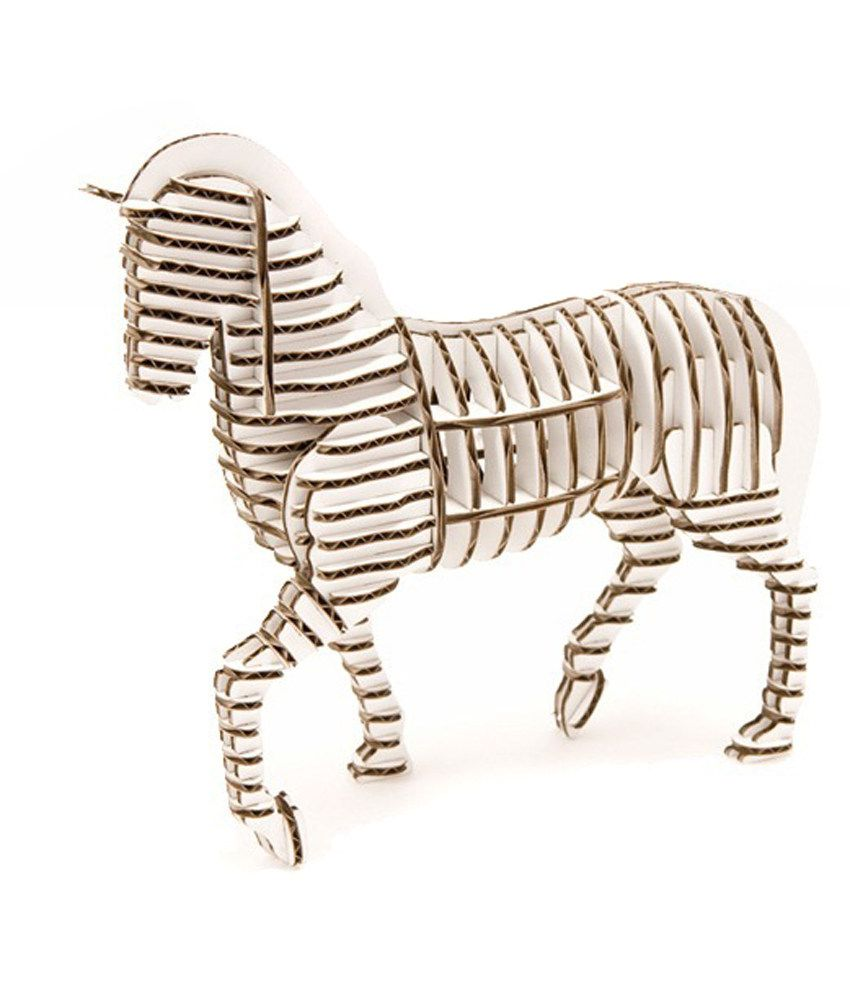
\includegraphics[width=0.2\linewidth]{modeling}
	\caption{}
	\label{fig:modeling}
\end{figure}
\end{frame}
\begin{frame}
	\frametitle{Configuration}
	$f_{\sigma_{1}(c_1)} \to f_{\sigma_{2}(c_1)}  \to f_{\sigma_{3}(c_1)}\quad (f_{\sigma_{1}(c_1)}=f_1,\quad f_{\sigma_{2}(c_1)=f_5},\quad f_{\sigma_{3}(c_1)}=f_8)$
	
	
\begin{figure}
	\centering
	\includegraphics[width=0.9\linewidth]{"Copy of Network Diagram Template"}
	\caption{
		Three configurations
	}
	\label{fig:copy-of-network-diagram-template}
\end{figure}
\end{frame}
\subsection{Objective function}
\begin{frame}
	\frametitle{Objective function}
	\begin{equation}
	\begin{split}
		min. \sum_{c\in C}\sum_{\hat{\gamma} \in \hat{\Gamma}_c} ( \sum_{sd \in SD} \sum_{\ell \in L} \sum_{i=1}^{n_c-1} b_{i \ell}^{\hat{\gamma}} \delta_{sd}^{\hat{\gamma}} delay_\ell)z_{\hat{\gamma}}+\\
		\sum_{c \in C} \sum_{\ell \in L} \sum_{sd \in SD} delay_\ell (y_\ell^{f_1(c),sd}+y_\ell^{f_{n_c}(c),sd})
		\end{split}
	\end{equation}
\begin{figure}
	\centering
	
\includegraphics[width=0.3\linewidth]{objective}
	\label{fig:objective}
\end{figure}	
\end{frame}
\subsection{Constrants}
\begin{frame}
	\frametitle{Constrants}
	\begin{equation}
		\sum_{\hat{\gamma} \in \hat{\Gamma}_c} \leq I_c \quad c \in C	
	\end{equation}
	\begin{equation}
		\sum_{v \in V}x_{vf} \leq R_f  \quad f \in F
	\end{equation}
	\begin{equation}
	\begin{split}
		\sum_{c \in C} \sum_{\hat{\gamma}\in \hat{\Gamma}_c}\sum_{sd \in SD}D_{sd}^{c} \delta^{\hat{\gamma}}_{sd}*\\
		(\sum_{f \in F} \sum_{i=1}^{n_c}T_{fi}^c n_f^{CORE} a_{vi}^{\hat{\gamma}})z_{\hat{\gamma}} \leq n_v^{FOGCORE}\quad v \in V_{FOG}
    \end{split}
	\end{equation}
	
\begin{figure}
	\centering
	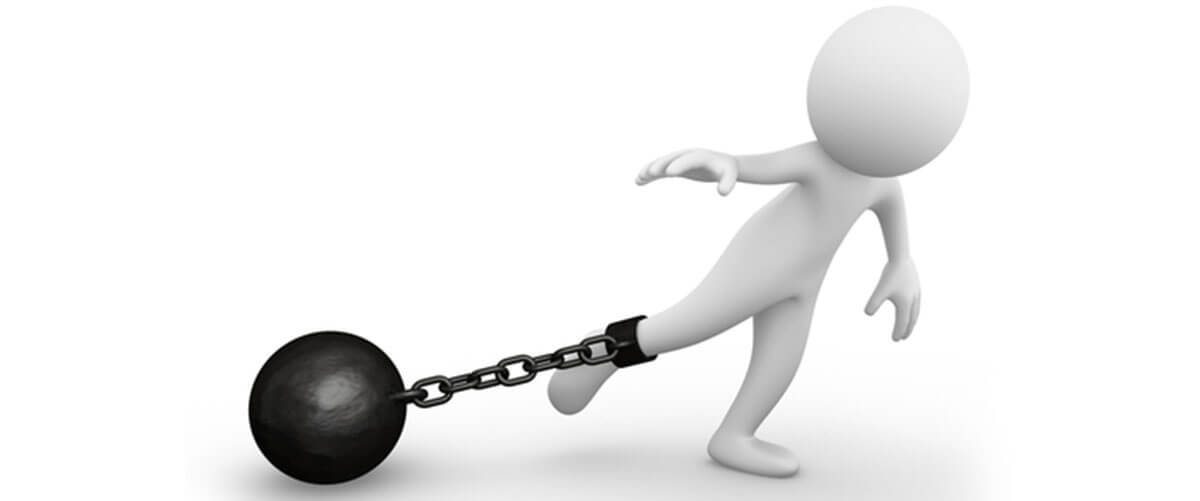
\includegraphics[width=0.4\linewidth]{constraints}
	\label{fig:constraints}
\end{figure}
\end{frame}
\begin{frame}
	\frametitle{Constrants}
	\onslide<+->{
		\begin{equation}
		\begin{split}
		\sum_{c \in C} \sum_{\hat{\gamma}\in \hat{\Gamma}_c}\sum_{sd \in SD}D_{sd}^{c} \delta^{\hat{\gamma}}_{sd}*\\
		(\sum_{f \in F} \sum_{i=1}^{n_c}T_{fi}^c n_f^{CORE} a_{vi}^{\hat{\gamma}})z_{\hat{\gamma}} \leq n_v^{CLOUDCORE}\quad v \in V_{CLOUD}
		\end{split}
		\end{equation}}
	%\onslide<+->{
		\begin{equation}
		\begin{split}
		\sum_{c \in C} \sum_{\hat{\gamma}\in \hat{\Gamma}_c}\sum_{sd \in SD}D_{sd}^{c}*\\
		(y_\ell^{f_1(c),sd}+y_\ell^{f_{n_c(c),sd}}+\sum_{\hat{\gamma \in \hat{\Gamma}_c}} \delta_{sd}^{\hat{\gamma}}z_{\hat{\gamma}}\sum_{i=1}^{n_cb-1b_{i \ell}^{\hat{\gamma}}}) \leq CAP_\ell
		\end{split}
		\end{equation}
%	}

\end{frame}
\begin{frame}
	\begin{equation}
	\begin{split}
	\sum_{\hat{\gamma} \in \hat{\Gamma}_c}\sum_{\ell \in L}delay_\ell*\\
	(y_\ell^{f_1(c),sd}+y_\ell^{f_{n_c(c),sd}}+\\
	\sum_{\hat{\gamma} \in \hat{\gamma}_c}\delta_{sd}^{\hat{\gamma}}z_{\hat{\gamma}}\sum_{i=1}^{n_c-1}b_{i\ell}^{\hat{\gamma}}\leq SLA_{sd}^c \quad c \in C , sd \in SD
	\end{split}
	\end{equation}
		\begin{equation}
	\begin{split}
	\sum_{\hat{\gamma} \in \hat{\Gamma}_c}\delta_{sd}^{\hat{\gamma}}z_{\hat{\gamma}}=1\quad c \in C , sd \in SD:D_{sd}^c>0
	\end{split}
	\end{equation}
	
\begin{figure}
	\centering
	
\includegraphics[width=0.3\linewidth]{constraints3}
	\label{fig:constraints3}
\end{figure}
\end{frame}
\section{Numeric Results}
\begin{frame}
\frametitle{Numeric Results}
\begin{itemize}
	\item {10 node pairs}
	\item {each VNF uses one core to run}
	\item {Each traffic	flow is 1Gbps} 
\end{itemize}	
	\begin{table}
		\begin{tabular}{|c|c|}
			\toprule
			\textbf{Service Chain} & \textbf{Chained VNFs}\\
			\midrule
			Online Gaming&NAT-FW-VOC-WOC-IDPS\\
			\hline
		\end{tabular}
	\end{table}

\begin{figure}
	\centering
	
\includegraphics[width=0.6\linewidth]{results}
	\label{fig:results}
\end{figure}
\end{frame}
\begin{frame}
	\frametitle{Numeric Results}
	
\begin{figure}
	\centering
	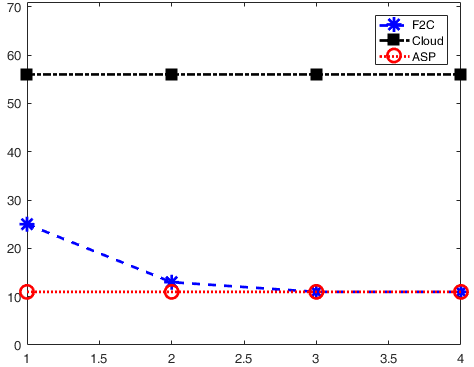
\includegraphics[width=0.6\linewidth]{Result}
	\caption{The overall end-to-end latency of network vs. number of instances.}
	\label{fig:result}
\end{figure}
\end{frame}
\section{Conclution}
\begin{frame}
\frametitle{Conclution}
	\begin{itemize}
		\item {multi Service
		Function Chain (SFC) mapping}
		\item {multiple SFC instances}
		\item {fog-to-cloud architecture}
		\item {formulate our problem as an Integer Linear
			Program}
		\item {minimize the overall end-to-end latency}
		\item {our model can achieve the least overall end-to-end latency
			when the number of instances increases}
	\end{itemize}
\begin{figure}
	\centering
	
\includegraphics[width=0.7\linewidth]{conclution}
	\caption{}
	\label{fig:conclution}
\end{figure}

\end{frame}
\begin{frame}
\frametitle{References}
[7] Drãxler, S., H. Karl, and Z.Á. Mann. Joint Optimization of Scaling and
Placement of Virtual Network Services. in 2017 17th IEEE/ACM
International Symposium on Cluster, Cloud and Grid Computing
(CCGRID). 2017.\\
$[8]$ Huin, N., B. Jaumard, and F. Giroire, Optimal Network Service Chain
Provisioning. IEEE/ACM Transactions on Networking, 2018. 26(3): p.
1320-1333.\\
$[9]$ Masri, W., et al. Minimizing delay in IoT systems through collaborative
fog-to-fog (F2F) communication. in 2017 Ninth International
Conference on Ubiquitous and Future Networks (ICUFN). 2017\\
$[10]$ Fan, J., et al. Deadline-Aware Task Scheduling in a Tiered IoT.Infrastructure. in GLOBECOM 2017 - 2017 IEEE Global Communications Conference. 2017.\\
$[11]$ Gupta, A., et al. Service Chain (SC) Mapping with Multiple SC
Instances in a Wide Area Network. in GLOBECOM 2017 - 2017 IEEE
Global Communications Conference. 2017.
\end{frame}
\begin{frame}
	
\begin{figure}
	\centering
	
\includegraphics[width=0.7\linewidth]{thanks}
		\label{fig:thanks}
\end{figure}
\end{frame}
\end{document} 